\documentclass[11pt,class=report,crop=false]{standalone}
\usepackage[screen]{../python}


\begin{document}

%====================================================================
\chapitre{Images et matrices}
%====================================================================

\index{image}
\index{matrice}

\objectifs{Le traitement des images est très utile, par exemple pour les agrandir ou bien les tourner. Nous allons aussi voir comment rendre une image plus floue, mais aussi plus nette ! Tout cela à l'aide des matrices.}


\bigskip

%%%%%%%%%%%%%%%%%%%%%%%%%%%%%%%%%%%%%%%%%%%%%%%%%%%%%%%%%%%%%%%%
%%%%%%%%%%%%%%%%%%%%%%%%%%%%%%%%%%%%%%%%%%%%%%%%%%%%%%%%%%%%%%%%

\begin{cours}[Convolution de matrices]

\index{convolution}

La convolution est l'action d'une matrice $C$ de taille $3\times 3$ sur un matrice $M$ de taille quelconque et qui transforme la matrice $M$ en une matrice $N$ de même taille. 

\begin{itemize}
\item \textbf{Principe.}
Pour chaque élément $m_{ij}$ de la matrice $M$ de départ, on regarde la sous-matrice $3\times3$ qui entoure cet élément (en gris foncé ci-dessous), on va multiplier ces éléments par les éléments de la matrice $C$, tout ceci va donner un seul élément : le coefficient $n_{ij}$ de la matrice $N$. 

\medskip

\myfigure{1}{\tikzinput{fig-matrice-1}}


\item \textbf{\'Elément de convolution.}
Voici comment calculer un élément de convolution. 
On multiplie chaque élément de la sous-matrice $3\times 3$ de $M$ par l'élément correspondant de $C$. La somme de ses produits donne l'élément de convolution :
$$n_{ij} = c_{00}a_{00} + c_{01}a_{01} + \cdots + c_{22}a_{22}$$

\medskip

\myfigure{1}{\tikzinput{fig-matrice-2}}

\item \textbf{Matrice obtenue.}
On calcule donc la matrice $N$ coefficient par coefficient, à chaque coefficient (symbolisés par un cercle) correspond donc une sous matrice $3\times 3$ de la matrice  $M$ (figure ci-dessous à gauche). Comment faire pour les coefficients qui sont au bord de la matrice ?
Si la sous-matrice déborde à droite elle repart à gauche (figure du centre), si elle 
déborde en bas, elle repart en haut, etc.

\myfigure{1}{\tikzinput{fig-matrice-3}}

Si on ne tenait pas compte des contraintes de bords, les coefficients de la sous-matrice autour du coefficient $m_{ij}$ seraient donnés par la sous-matrice ci-dessous à gauche, mais pour tenir compte des débordements on raisonne à l'aide des modulos (sous-matrice de droite). Les indices $i$ des lignes sont calculés modulo $n$ (où $n$ est le nombre de lignes de la matrice $M$), les indices $j$ des colonnes sont calculés modulo $p$ (où $p$ est le nombre de colonnes de la matrice $M$)  :
\myfigure{1}{\tikzinput{fig-matrice-4}}


\item Exemple.

$$M = \begin{pmatrix}
1&2&3&4\\5&6&7&8\\9&10&11&12\\
\end{pmatrix}\qquad
C = \begin{pmatrix}
0&1&0\\1&2&1\\0&1&0\\
\end{pmatrix}\qquad
N = \begin{pmatrix}
22 & 24 & 30 & 32 \\ 
34 & 36 & 42 & 44 \\ 
46 & 48 & 54 & 56 \\
\end{pmatrix}$$

\smallskip

Par exemple voici le calcul du coefficient $n_{11}$ :
$$n_{11} = c_{00}m_{00} + c_{01}m_{01} + \cdots + c_{22}m_{22}
= 0\times 1 + 1\times 2 + 0 \times 3 
+ 1\times 5 + 2\times 6 + 1 \times 7   
+ 0\times 9 + 1\times 10 + 0 \times 11 = 36
$$

\end{itemize}
\end{cours}

%%%%%%%%%%%%%%%%%%%%%%%%%%%%%%%%%%%%%%%%%%%%%%%%%%%%%%%%%%%%%%%%
%%%%%%%%%%%%%%%%%%%%%%%%%%%%%%%%%%%%%%%%%%%%%%%%%%%%%%%%%%%%%%%%

\begin{cours}[Modélisation de matrices]
\sauteligne	
	\begin{itemize}
		\item Une matrice est codée par un tableau, c'est-à-dire une liste de listes.
		Par exemple :		
		\mycenterline{\ci{M = [[1,2,3,4], [5,6,7,8], [9,10,11,12]]}}
		représente la matrice :
		$$M = \begin{pmatrix}
		1&2&3&4\\5&6&7&8\\9&10&11&12\\
		\end{pmatrix}$$
		
		\item On accède à l'élément $(i,j)$ par :		
		\mycenterline{\ci{M[i][j]}}
		
		
		\item Une matrice $M$ de $n$ lignes et $p$ colonnes est donc une liste de longueur $n$, chaque élément étant une liste de longueur $p$ :		
		\mycenterline{\ci{n = len(M)} \qquad \ci{p = len(M[0])}}
		
		\item Comme d'habitude la numérotation commence à $0$, donc $0 \le i < n$ et $0 \le j < p$.
		
		\item On initialise une matrice avec des coefficients nuls ainsi :		
		\mycenterline{\ci{M = [[0 for j in range(p)] for i in range(n)]}}
		
		On peut ensuite remplir la matrice coefficient par coefficient par des commandes du type :		
		\mycenterline{\ci{M[i][j] = ...}}
	\end{itemize}

\end{cours}

%%%%%%%%%%%%%%%%%%%%%%%%%%%%%%%%%%%%%%%%%%%%%%%%%%%%%%%%%%%%%%%%
% Activité 1 - Convolution de matrices
%%%%%%%%%%%%%%%%%%%%%%%%%%%%%%%%%%%%%%%%%%%%%%%%%%%%%%%%%%%%%%%%

\begin{activite}[Convolution de matrices]
	
\objectifs{Objectifs : calculer une convolution.}
		
\begin{enumerate}
	\item Programme une fonction \ci{afficher_matrice(M)} qui réalise un affichage propre d'une matrice sur le terminal de l'écran.
	

	Voici un exemple d'affichage :
	
\begin{center}
	\begin{minipage}{0.55\textwidth}
	\begin{center}
	\begin{lstlisting}
	M = [[1,2,3], [4,5,6], [7,8,9]]	
	\end{lstlisting}		
	\end{center}	
	\end{minipage}\qquad\qquad
	\begin{minipage}{0.4\textwidth}
	\begin{center}
	\begin{lstlisting}
	1   2   3 
	4   5   6 
	7   8   9	
	\end{lstlisting}
	\end{center}
	\end{minipage}
\end{center}



	\emph{Indications.}
	\begin{itemize}
		\item \ci{print('\{:3d\}'.format(x),end=" ")} affiche un entier sur $3$ caractères.
		\item \ci{print('\{0:.3f\}'.format(x),end=" ")} affiche un nombre flottant avec $3$ décimales après la virgule.
	\end{itemize}
			
	\item Programme une fonction \ci{element_convolution(C,M)} qui à partir de deux matrices $C$ et $M$ de taille $3\times 3$ calcule l'élément de convolution :
	$$\gamma = c_{00}m_{00} + c_{01}m_{01} + \cdots + c_{22}m_{22}$$
	Autrement dit $\gamma$ est la somme des produits des coefficients entre $C$ et $M$.
	Par exemple pour :	
	\mycenterline{\ci{C = [[1,1,1], [1,5,1], [1,1,1]]}}	
	\mycenterline{\ci{M = [[1,2,3], [4,5,6], [7,8,9]]}}
	L'élément de convolution est $$\gamma = 1\times 1 + 1\times 2 + 	1\times 3 + 1\times 4 + 5 \times 5 + 1\times 6 + 1\times 7 + 	1\times 8 + 1\times 9 = 65.$$

	\item Programme une fonction \ci{convolution(C,M)} qui calcule la matrice $N$ de convolution de $C$ sur $M$.
	\begin{itemize}
		\item $C$ est une matrice $3\times 3$.
		\item $M$ est une matrice de taille quelconque $n\times p$.
		\item $N = \text{convolution}(C,M)$ est aussi de taille $n \times p$ et chaque coefficient $n_{ij}$ est l'élément de convolution de $C$ avec $M'_{ij}$ la sous-matrice $3\times 3$ de $M$ autour du coefficient en $(i,j)$.
		\item N'oublie pas que pour la sous-matrice il y a des effets de bords (voir les formules avec les modulos dans le cours ci-dessus).
	\end{itemize}
	Par exemple 
	$$
	C = \begin{pmatrix}0&1&0\\0&0&0\\0&0&0\end{pmatrix}\qquad
	M = \begin{pmatrix}1&2&3&4\\5&6&7&8\\9&10&11&12\end{pmatrix}\qquad	
	\text {donnent} \qquad
	N = \begin{pmatrix}9&10&11&12\\1&2&3&4\\5&6&7&8\end{pmatrix}$$
	Avec cette matrice $C$, la convolution sur $M$ correspond à faire descendre chaque coefficient d'une ligne (et comme on travaille avec les modulos, un coefficient de la dernière ligne se retrouve sur la première ligne).
	
	
	\item Utilise ou modifie la fonction précédente en une fonction \ci{convolution_entiere(C,M)} qui renvoie une matrice dont les coefficients sont arrondis à des entiers, limités à $255$, les coefficients négatifs étant ramenés à zéros.
	
	Exemple.
	$$
	C = \begin{pmatrix}0&-\frac12&0\\-\frac12&3&-\frac12\\0&-\frac12&0\end{pmatrix}\qquad
	M = \begin{pmatrix}
	101&102&103&104\\
	201&151&101&51\\
	50&100&150&200
	\end{pmatrix}$$
	donnent la convolution $N$ et la convolution entière $N'$ :
	$$N = \begin{pmatrix}
	74.5&78.5&80.5&84.5\\ 
	426.5&201.0&75.5&-150.0\\
	-151.0&73.5&198.0&422.5
	\end{pmatrix}
	\qquad \text{ et } \qquad 
	N'= \begin{pmatrix}
		74&78&80&84\\ 
		255&201&75&0\\
		0&73&198&255
	\end{pmatrix}$$
	
\end{enumerate}
		
\end{activite}


%%%%%%%%%%%%%%%%%%%%%%%%%%%%%%%%%%%%%%%%%%%%%%%%%%%%%%%%%%%%%%%%
%%%%%%%%%%%%%%%%%%%%%%%%%%%%%%%%%%%%%%%%%%%%%%%%%%%%%%%%%%%%%%%%

\begin{cours}[Format d'image \og{}pgm\fg{}]
	

\index{pgm@\emph{pgm}}

Le format d'image \og{}pgm\fg{}	est un format très simple de fichier texte qui permet de décrire une image.
Voici un exemple très simple : à gauche le fichier et à droite l'image correspondante.

\begin{center}
\begin{minipage}{0.4\textwidth}
\begin{lstlisting}
P2
5 4
255
  0 255  64 255   0
255   0 127   0 255
 64 127   0 127  64
255   0 127   0 255
\end{lstlisting}
\end{minipage}	
\begin{minipage}{0.4\textwidth}
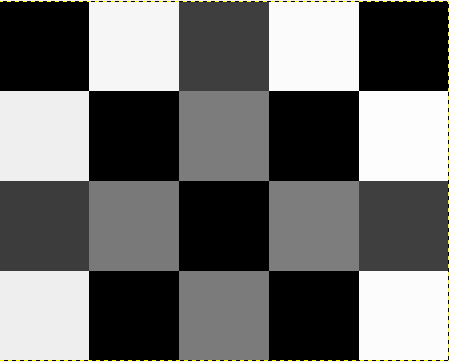
\includegraphics[scale=\myscale,scale=0.3]{ecran-cours-pgm}
\end{minipage}
\end{center}

\textbf{Explications.}
\begin{itemize}
	\item \ci{P2} est le code pour le format d'image en niveau de gris (\ci{P1} désigne les images en noir et blanc, \ci{P3} les images en couleurs).
	\item Les entiers $5$ et $4$ sont le nombre de colonnes suivi du nombre de lignes de l'image (ici $5$ colonnes et $4$ lignes).
	\item $255$ désigne le découpage en niveau de gris : ici de $0$ (noir) à $255$ (blanc).
	\item Les entiers suivants sont le niveau de gris de chacun des pixels de l'image.
\end{itemize}

\bigskip

\textbf{Version étendue.}	
Ce format d'image est reconnu par tous les bons lecteurs d'images. Les logiciels de retouches d'images permettent d'exporter n'importe quelle image vers ce format. Par contre la structure du fichier peut être différente : tout d'abord il peut y avoir des lignes de commentaires (commençant par \#), ensuite les valeurs de niveau de gris de chaque pixel peuvent être toutes sur une même ligne ou bien un seul pixel par ligne.
C'est par exemple le cas du logiciel \emph{gimp} qui produit des fichiers comme ci-dessous à gauche.

\begin{center}
\begin{minipage}{0.4\textwidth}
\begin{lstlisting}
P2
# Commentaire !
5 4
255
0
255
64
255
0
255
...
\end{lstlisting}
\end{minipage}	
\begin{minipage}{0.4\textwidth}
\begin{lstlisting}
P2
5 4
255
0 255 64 255 0 255 0 127 ...
\end{lstlisting}
\end{minipage}
\end{center}

\end{cours}


%%%%%%%%%%%%%%%%%%%%%%%%%%%%%%%%%%%%%%%%%%%%%%%%%%%%%%%%%%%%%%%%
% Activité 2 - Lire et écrire des images
%%%%%%%%%%%%%%%%%%%%%%%%%%%%%%%%%%%%%%%%%%%%%%%%%%%%%%%%%%%%%%%%

\begin{activite}[Lire et écrire des images]
	
\objectifs{Objectifs : convertir un fichier d'image en une matrice et inversement.}
	
	
\begin{enumerate}
	\item Programme une fonction \ci{pgm_vers_matrice(fichier)}
	qui lit un fichier d'image au format \og{}pgm\fg{} dont le nom est donné et renvoie une matrice. 
	
	Voici un exemple de fichier et la matrice associée :
\begin{center}
\begin{minipage}{0.4\textwidth}
\begin{lstlisting}
P2
4 5
255
  0   0   0   0
  0 255 255   0
  0 128 128   0
255 255 255 255
  0  64  64   0
\end{lstlisting}
\end{minipage}
\begin{minipage}{0.4\textwidth}
$$\begin{pmatrix}
   0 &   0 &   0 &   0 \\
0 & 255 & 255 &   0 \\
0 & 128 & 128 &   0 \\
255 & 255 & 255 & 255 \\
0 &  64 &  64 &   0 \\
\end{pmatrix}$$
\end{minipage}	
\end{center}

	C'est préférable si ta fonction accepte les fichiers au format \og{}pgm\fg{} étendu qui peuvent contenir des commentaires et où il n'y a qu'une nuance de gris par ligne. (Voir le cours ci-dessus.)
		
	\item Fais le travail inverse en programmant une fonction \ci{matrice_vers_pgm(M,fichier)} qui part d'une matrice $M$ et écrit un fichier (dont le nom est donné) au format \og{}pgm\fg{}.
		
\end{enumerate}

\end{activite}



%%%%%%%%%%%%%%%%%%%%%%%%%%%%%%%%%%%%%%%%%%%%%%%%%%%%%%%%%%%%%%%%
% Activité 3 - Convolution d'une image
%%%%%%%%%%%%%%%%%%%%%%%%%%%%%%%%%%%%%%%%%%%%%%%%%%%%%%%%%%%%%%%%

\begin{activite}[Convolution d'une image]
	
\objectifs{Objectifs : appliquer la convolution pour transformer une image.}
	
\begin{center}
	\begin{minipage}{0.18\textwidth}\center
		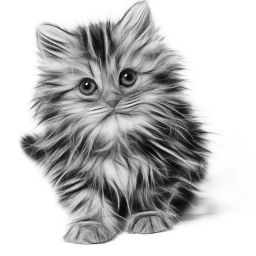
\includegraphics[scale=\myscale,scale=0.3]{png/chat}
		
		Image originale
	\end{minipage}
	\begin{minipage}{0.18\textwidth}\center
		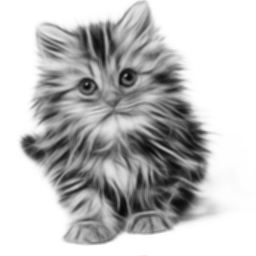
\includegraphics[scale=\myscale,scale=0.3]{png/chat_conv_flou}
		\newline Flou
	\end{minipage}
	\begin{minipage}{0.18\textwidth}\center
		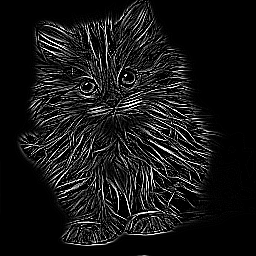
\includegraphics[scale=\myscale,scale=0.3]{png/chat_conv_bord}
		
		Bords
	\end{minipage}
	\begin{minipage}{0.18\textwidth}\center
		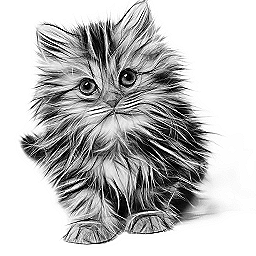
\includegraphics[scale=\myscale,scale=0.3]{png/chat_conv_pique}
		
		Piqué
	\end{minipage}
	\begin{minipage}{0.18\textwidth}\center
		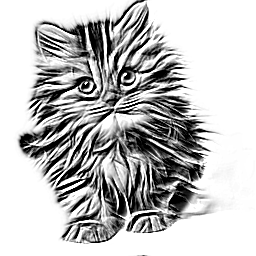
\includegraphics[scale=\myscale,scale=0.3]{png/chat_conv_estampe}
		
		Estampé
	\end{minipage}	
\end{center}	
	
	
Programme une fonction \ci{convolution_image(C,fichier_in,fichier_out)}
qui à partir d'une matrice de convolution $C$ de taille $3\times3$ et d'une image (dont le nom est donné) écrit les éléments d'une nouvelle image dans un fichier (dont le nom est aussi donné). Les fichiers d'images sont au format \og{}pgm\fg{}.

C'est une fonction très simple qui utilise la fonction \ci{convolution_entiere()}.
Ensuite teste différentes convolutions !

\bigskip

\textbf{Flou.}
La convolution avec la matrice suivante \og{}floute\fg{} légèrement l'image.
C'est parce que le niveau de gris de chaque nouveau pixel est la moyenne des niveaux des $9$ pixels voisins de l'image de départ.
$$C = 
\begin{pmatrix}
\frac19&\frac19&\frac19\\
\frac19&\frac19&\frac19\\
\frac19&\frac19&\frac19
\end{pmatrix}$$

\begin{center}
	\begin{minipage}{0.45\textwidth}\center
	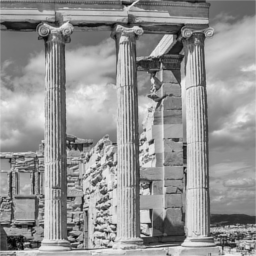
\includegraphics[scale=\myscale,scale=0.5]{png/colonnes}
	
	Image originale
	\end{minipage}
	\begin{minipage}{0.45\textwidth}\center
	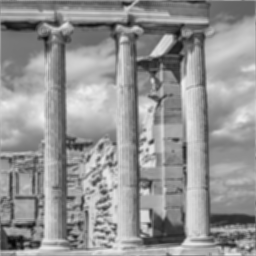
\includegraphics[scale=\myscale,scale=0.5]{png/colonnes_conv_flou}
	
	Flou
    \end{minipage}	
\end{center}


Essaye aussi le \emph{flou gaussien} avec la matrice : 
$$C = 
\begin{pmatrix}
\frac1{16}&\frac2{16}&\frac1{16}\\
\frac2{16}&\frac4{16}&\frac2{16}\\
\frac1{16}&\frac2{16}&\frac1{16}
\end{pmatrix}$$


\bigskip

\textbf{Bords.}

$$C = 
\begin{pmatrix}
-1&-1&-1\\
-1&8&-1\\
-1&-1&-1\\
\end{pmatrix}$$


\begin{center}
	\begin{minipage}{0.45\textwidth}\center
		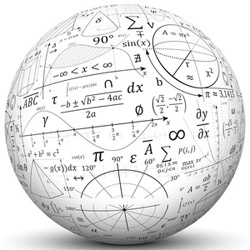
\includegraphics[scale=\myscale,scale=0.5]{png/monde}
		
		Image originale
	\end{minipage}
	\begin{minipage}{0.45\textwidth}\center
		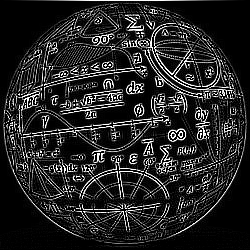
\includegraphics[scale=\myscale,scale=0.5]{png/monde_conv_bord}
		
		Bords
	\end{minipage}	
\end{center}

Essaie aussi les matrices : 
$$C = 
\begin{pmatrix}
0&1&0\\
1&-4&1\\
0&1&0\\
\end{pmatrix} \qquad \text{ ou } \qquad
C = \begin{pmatrix}
1&0&-1\\
0&0&0\\
-1&0&1\\
\end{pmatrix}$$


\bigskip

\textbf{Piqué.}

C'est le contraire du flou !

$$C = 
\begin{pmatrix}
0&-1&0\\
-1&5&-1\\
0&-1&0\\
\end{pmatrix}$$

Voici un exemple avec l'image originale à gauche et l'image transformée à droite qui a l'air plus nette que l'originale !
\begin{center}
	\begin{minipage}{0.45\textwidth}\center
		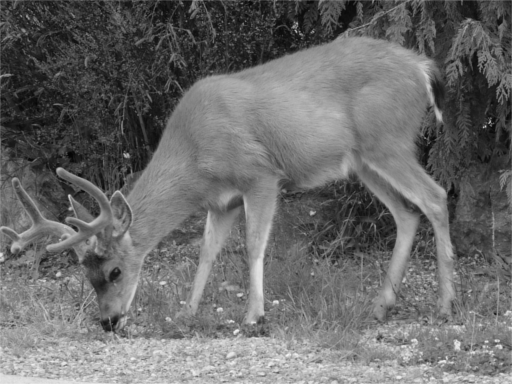
\includegraphics[scale=\myscale,scale=0.3]{png/renne}
		
		Image originale
	\end{minipage}
	\begin{minipage}{0.45\textwidth}\center
		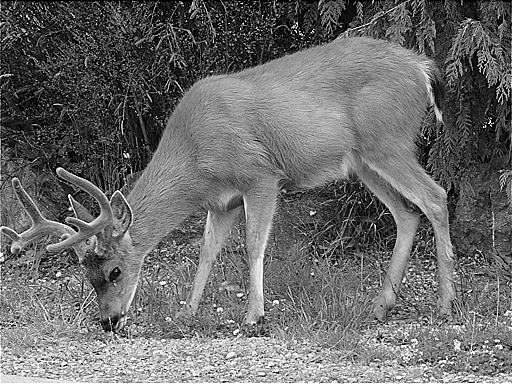
\includegraphics[scale=\myscale,scale=0.3]{png/renne_conv_pique}
		
		Piqué
	\end{minipage}	
\end{center}

\bigskip

\textbf{Estampé.}

$$C = 
\begin{pmatrix}
-2&-1&0\\
-1&1&1\\
0&1&2\\
\end{pmatrix}$$


\begin{center}
	\begin{minipage}{0.45\textwidth}\center
		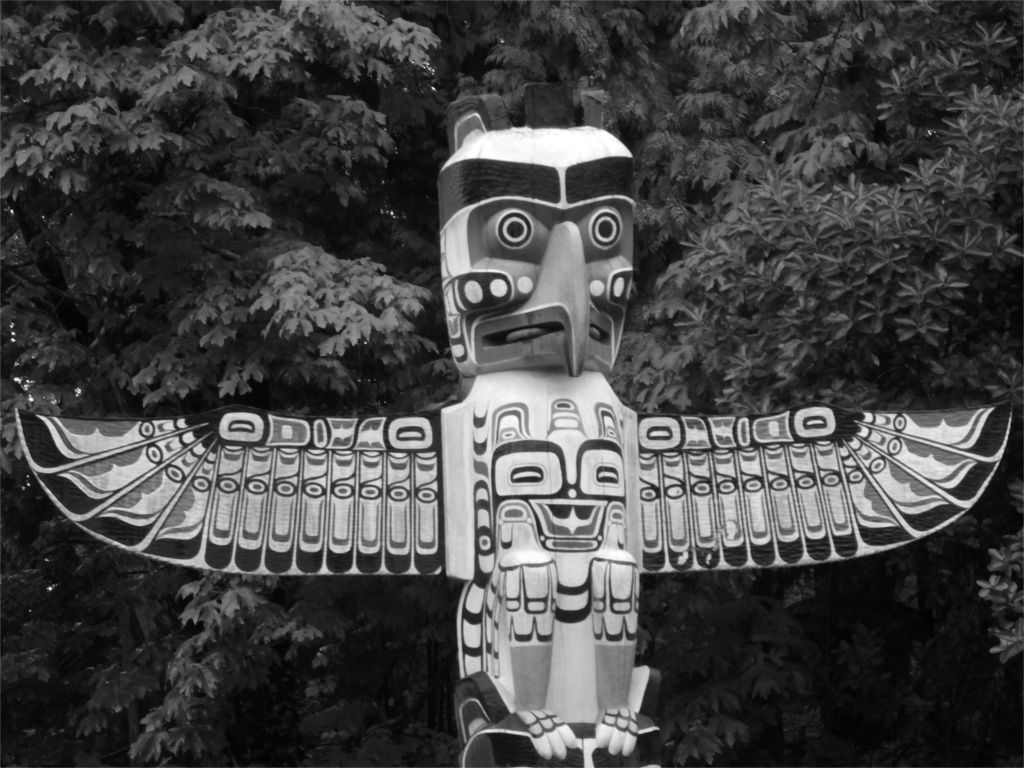
\includegraphics[scale=\myscale,scale=0.18]{png/totem}
		 
		Image originale
	\end{minipage}
	\begin{minipage}{0.45\textwidth}\center
		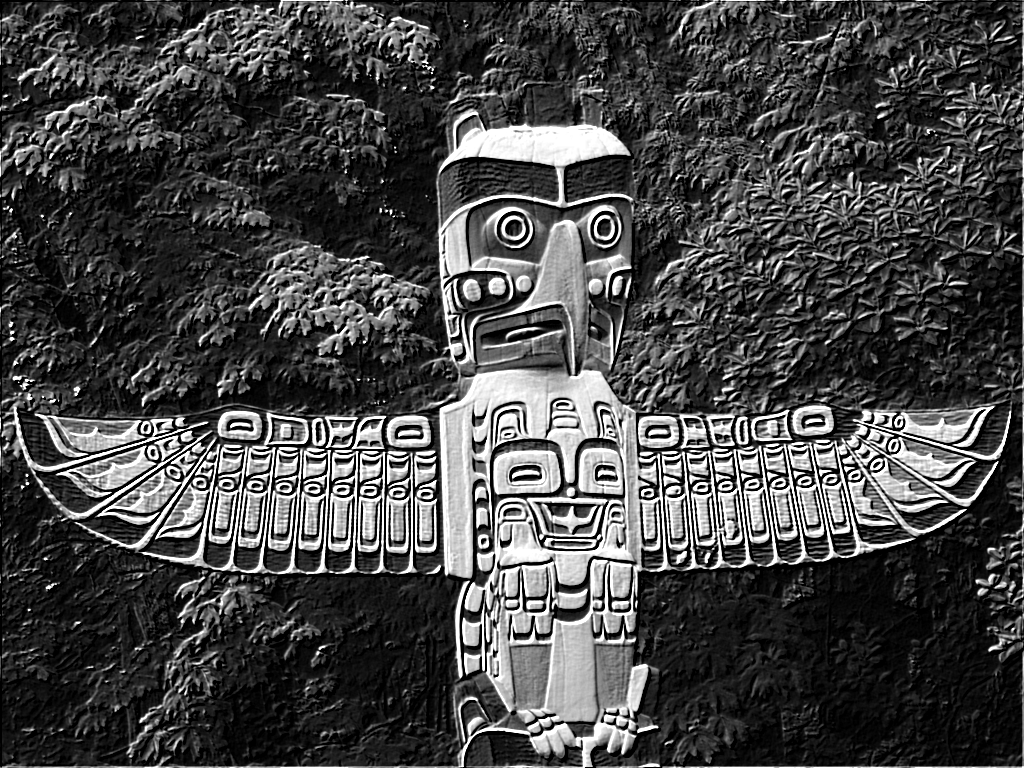
\includegraphics[scale=\myscale,scale=0.18]{png/totem_conv_estampe}
		
		Estampé
	\end{minipage}	
\end{center}



\bigskip

\textbf{Décalage vers le haut.}

Trouve la convolution qui décale l'image d'un pixel vers le haut et permet d'obtenir l'image suivante par itération.
\begin{center}
		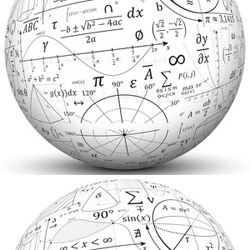
\includegraphics[scale=\myscale,scale=0.55]{png/monde_conv_decal}
		
		Décalage itéré vers le haut
\end{center}
		
\end{activite}

%%%%%%%%%%%%%%%%%%%%%%%%%%%%%%%%%%%%%%%%%%%%%%%%%%%%%%%%%%%%%%%%
%%%%%%%%%%%%%%%%%%%%%%%%%%%%%%%%%%%%%%%%%%%%%%%%%%%%%%%%%%%%%%%%

\begin{cours}[Matrice de transformation]
Voici de brefs rappels sur les matrices en se limitant aux matrices $2\times 2$. Pour l'interprétation géométrique, on identifie un point $P$ de coordonnées $(x,y)$ avec le vecteur $\vec u = \left(\begin{smallmatrix}x\\y\\\end{smallmatrix}\right)$.

\begin{itemize}
	\item \textbf{Multiplication par un vecteur.}
	$$X = \begin{pmatrix}x\\y\\	\end{pmatrix}\quad \text{ et } \quad
	M = \begin{pmatrix}	a & b \\	c & d \\\end{pmatrix}
	\qquad \text{ alors } \qquad
	X' = A X = \begin{pmatrix}ax+by\\cx+dy\\\end{pmatrix}$$
	
	Autrement dit, les coordonnées $(x',y')$ de l'image de $P=(x,y)$ sont données par :
	$$\left\{\begin{array}{rcl}
	x' &=& ax+by\\
	y' &=& cx+dy\\
	\end{array}
	\right.$$	


\myfigure{0.8}{\tikzinput{fig-transfo-1}}	

\medskip

\myfigure{0.9}{\tikzinput{fig-transfo-2}}	


		
	\item \textbf{Matrice de rotation.}
	
	$$T_\theta = \begin{pmatrix}\cos \theta& -\sin \theta\\\sin\theta&\cos\theta\end{pmatrix}$$
	
	Autrement dit, pour $X'=T_\theta X$, on a : 
	$$\left\{\begin{array}{rcl}
	x' &=& x\cos \theta -y\sin \theta\\
	y' &=& x\sin\theta + y\cos\theta \\
	\end{array} \right.$$

\myfigure{0.9}{\tikzinput{fig-transfo-3}}		

\medskip

	\item \textbf{Dilatation.}
	
	$$T = \begin{pmatrix}k_x&0\\0&k_y\end{pmatrix}$$
	Autrement dit :
	$$\left\{\begin{array}{rcl}
	x' &=& k_x \cdot x\\
	y' &=& k_y \cdot y\\
	\end{array}\right.$$

Un exemple avec $k_x = 2$, $k_y = \frac12$.

\medskip

\myfigure{0.9}{\tikzinput{fig-transfo-4}}		

\medskip
			
	\item \textbf{Inverse.}
	Une matrice $M$, dont le déterminant est non nul, admet un inverse $M^{-1}$ :
	$$M = \begin{pmatrix}	a & b \\	c & d \\\end{pmatrix} \qquad
	M^{-1} = \frac{1}{ad-bc}\begin{pmatrix}d & -b \\-c & a \\\end{pmatrix}$$

\medskip
	
\myfigure{0.9}{\tikzinput{fig-transfo-5}}		
	
	
%	\item \textbf{Coordonnées mathématiques et coefficients des matrices.}
%	Il faut garder à l'esprit que les convention pour les coordonnées mathématiques $(x,y)$ et les coefficients des matrices $(i,j)$.
%
%
%\myfigure{0.7}{\tikzinput{fig-transfo-6}}		
	
\end{itemize}	

\end{cours}

%%%%%%%%%%%%%%%%%%%%%%%%%%%%%%%%%%%%%%%%%%%%%%%%%%%%%%%%%%%%%%%%
% Activité 4 - Transformation d'images
%%%%%%%%%%%%%%%%%%%%%%%%%%%%%%%%%%%%%%%%%%%%%%%%%%%%%%%%%%%%%%%%

\begin{activite}[Transformation d'images]
	
	\objectifs{Objectifs : utiliser les matrices pour tourner, inverser ou déformer une image.}
	
	
\begin{enumerate}
	\item \textbf{Dilatation.}
	
	Programme une fonction \ci{dilatation_matrice(kx,ky,M)} qui effectue une dilatation de la matrice $M$. La matrice est agrandie d'un facteur $k_x$ horizontalement et d'un facteur $k_y$ verticalement en une nouvelle matrice $N$ (ici $k_x$ et $k_y$ sont des entiers).
			
	\emph{Exemple.} Voici un exemple avec $k_x=3$ et $k_y=2$.
$$M = \begin{pmatrix}		
1 & 2 & 3 \\
4 & 5 & 6 \\
7 & 8 & 9 \\
\end{pmatrix} \qquad \text{ devient } \qquad
N = \begin{pmatrix}
1 & 1 & 1 & 2 & 2 & 2 & 3 & 3 & 3 \\
1 & 1 & 1 & 2 & 2 & 2 & 3 & 3 & 3 \\
4 & 4 & 4 & 5 & 5 & 5 & 6 & 6 & 6 \\
4 & 4 & 4 & 5 & 5 & 5 & 6 & 6 & 6 \\
7 & 7 & 7 & 8 & 8 & 8 & 9 & 9 & 9 \\
7 & 7 & 7 & 8 & 8 & 8 & 9 & 9 & 9 \\		
\end{pmatrix}$$

    \emph{Formule.}
    On obtient les coefficients de la nouvelle matrice $N$ en fonction des coefficients de l'ancienne matrice $M$ :
    $$N[i][j] = M[i//k_y][j//k_x]$$

	\emph{Indications.}
	\begin{itemize}
		\item Commence par initialiser une matrice vide :		
		\mycenterline{\ci{N = [[0 for j in range(kx*p)] for i in range(ky*n)]}}
		de la bonne taille.
		
		\item Prends garde que horizontalement $x$ correspond à $j$ et verticalement $y$ correspond à $i$.
		
	\end{itemize}
		
	\emph{Application.} Dilate des images.
	\begin{center}
	\begin{minipage}{0.3\textwidth}\center
		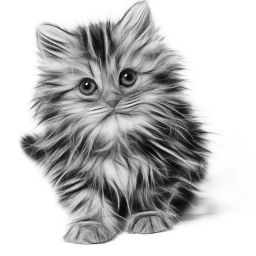
\includegraphics[scale=\myscale,scale=0.18]{png/chat}
		
		Image originale
	\end{minipage}
	\begin{minipage}{0.45\textwidth}\center
		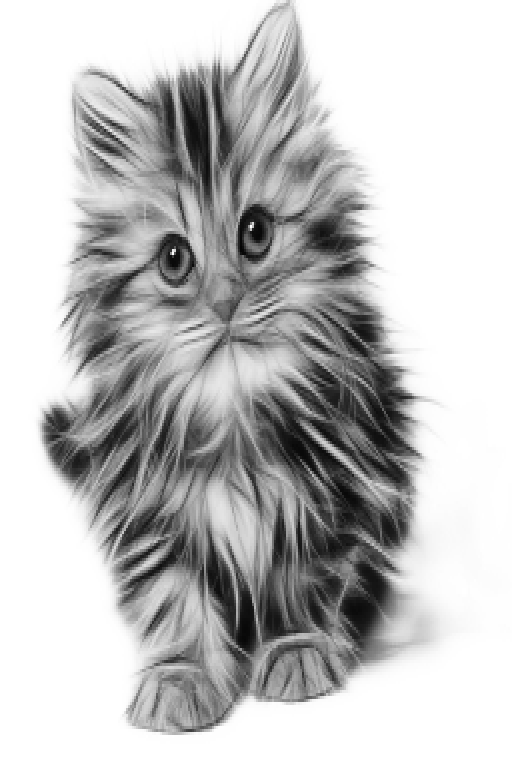
\includegraphics[scale=\myscale,scale=0.18]{png/chat_biho}
		
		Image dilatée $(k_x=2,k_y=3)$
	\end{minipage}	
	\end{center}
  	L'image dilatée est plus grande mais sa résolution est plus faible, au final il n'y a ni gain ni perte d'information.	
		
	\item \textbf{Matrice de transformation.}
	
	On souhaite généraliser la question précédente avec une transformation quelconque.
	\begin{itemize}
		\item Programme une fonction \ci{vecteur_image(T,x,y)} qui à partir d'une matrice de transformation $T$ et des coordonnées $\left(\begin{smallmatrix}x\\y\end{smallmatrix}\right)$ d'un vecteur renvoie les coordonnées $\left(\begin{smallmatrix}x'\\y'\end{smallmatrix}\right)$ de l'image de ce vecteur par $T$ :
		$$T = \begin{pmatrix}a&b\\c&d\end{pmatrix}\qquad\qquad
		\begin{pmatrix}x' \\ y' \end{pmatrix} = T \begin{pmatrix}x \\ y \end{pmatrix}
		= \begin{pmatrix}ax+by \\ cx+dy \end{pmatrix}$$
		
		\item Programme une fonction \ci{inverse_matrice(T)} qui renvoie la matrice inverse de la matrice $T$ (dont on suppose le déterminant non nul).
		$$T = \begin{pmatrix}a&b\\c&d\end{pmatrix}
		\qquad \qquad
		T^{-1} = \frac{1}{ad-bc}\begin{pmatrix}d&-b\\-c&a\end{pmatrix}$$
		
		\item \emph{Application.}
		Soit $T_\theta$ la matrice de rotation d'angle $\theta$ :
		$$T_\theta = \begin{pmatrix}\cos \theta& -\sin \theta\\\sin\theta&\cos\theta\end{pmatrix}$$
		Soit $\theta = \frac\pi3$. Soit $P = (x,y) = (4,5)$. Calcule l'image de $P$ par la rotation d'angle $\theta$. C'est le point $P' = (x',y')$ dont les coordonnées sont obtenues par multiplication de $T_\theta$ par le vecteur $\left(\begin{smallmatrix}x\\y\end{smallmatrix}\right)$.
		
		\item \emph{Application.}
		Vérifie pour $\theta=\frac\pi3$ (par exemple) que la matrice de rotation
		$T_{-\theta}$ est égale à la matrice $(T_\theta)^{-1}$. (C'est juste une vérification par le calcul que l'opération inverse de tourner d'un angle $\theta$ c'est tourner d'un angle $-\theta$ !)
		
	\end{itemize}

	\item \textbf{Action de la transformation.}

	Le but est de programmer une fonction \ci{transformation(T,M)} qui à partir d'une matrice $T$ de taille $2\times 2$ transforme une matrice $M$ (de taille quelconque)
	en une nouvelle matrice $N$.
	
	\emph{Application.} Tu peux ensuite faire agir n'importe quelle matrice $T$ pour transformer une image.
	
	\begin{center}
	\begin{minipage}{0.5\textwidth}
		\textbf{Dilatation} (avec constantes quelconques).
		$$T = \begin{pmatrix}k_x&0\\0&k_y\end{pmatrix} \quad \text{ avec } k_x=\pi=3.14\ldots,\  k_y = 1$$	
	\end{minipage}
	\begin{minipage}{0.4\textwidth}\center
		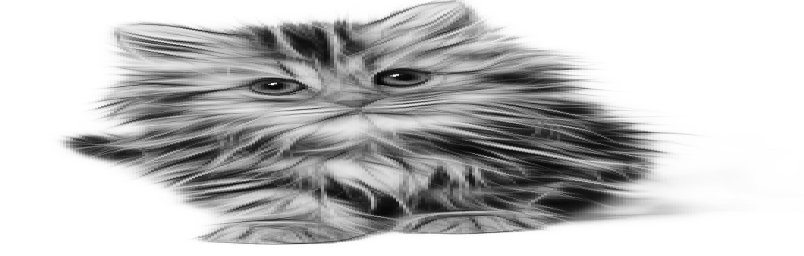
\includegraphics[scale=\myscale,scale=0.3]{png/chat_dilatation}
	\end{minipage}	
    \end{center}
	
	
	\begin{center}
		\begin{minipage}{0.4\textwidth}
		\textbf{Rotation.}
		
		$$T = \begin{pmatrix}\cos \theta& -\sin \theta\\\sin\theta&\cos\theta\end{pmatrix} \qquad \text{ avec } \theta = \frac\pi3$$	
		\end{minipage}
		\begin{minipage}{0.45\textwidth}\center
			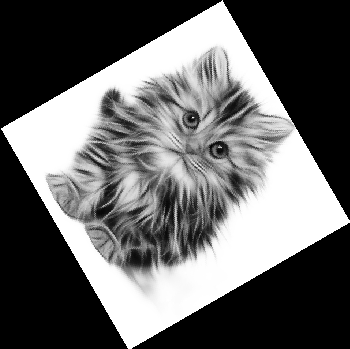
\includegraphics[scale=\myscale,scale=0.3]{png/chat_rotation}
		\end{minipage}	
	\end{center}

	\begin{center}
	\begin{minipage}{0.4\textwidth}
		\textbf{Symétrie.}
		
		$$T = \begin{pmatrix}1&0\\0&-1\end{pmatrix}$$	
	\end{minipage}
	\begin{minipage}{0.45\textwidth}\center
		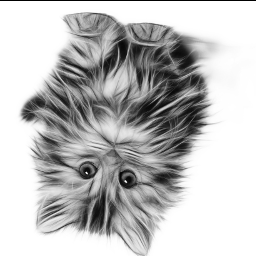
\includegraphics[scale=\myscale,scale=0.4]{png/chat_symetrie}
	\end{minipage}
	\end{center}

	\begin{center}
	\begin{minipage}{0.4\textwidth}
		\textbf{Transformation quelconque.}
		
		$$T = \begin{pmatrix}3&1\\1&5\end{pmatrix}$$	
	\end{minipage}
	\begin{minipage}{0.45\textwidth}\center
		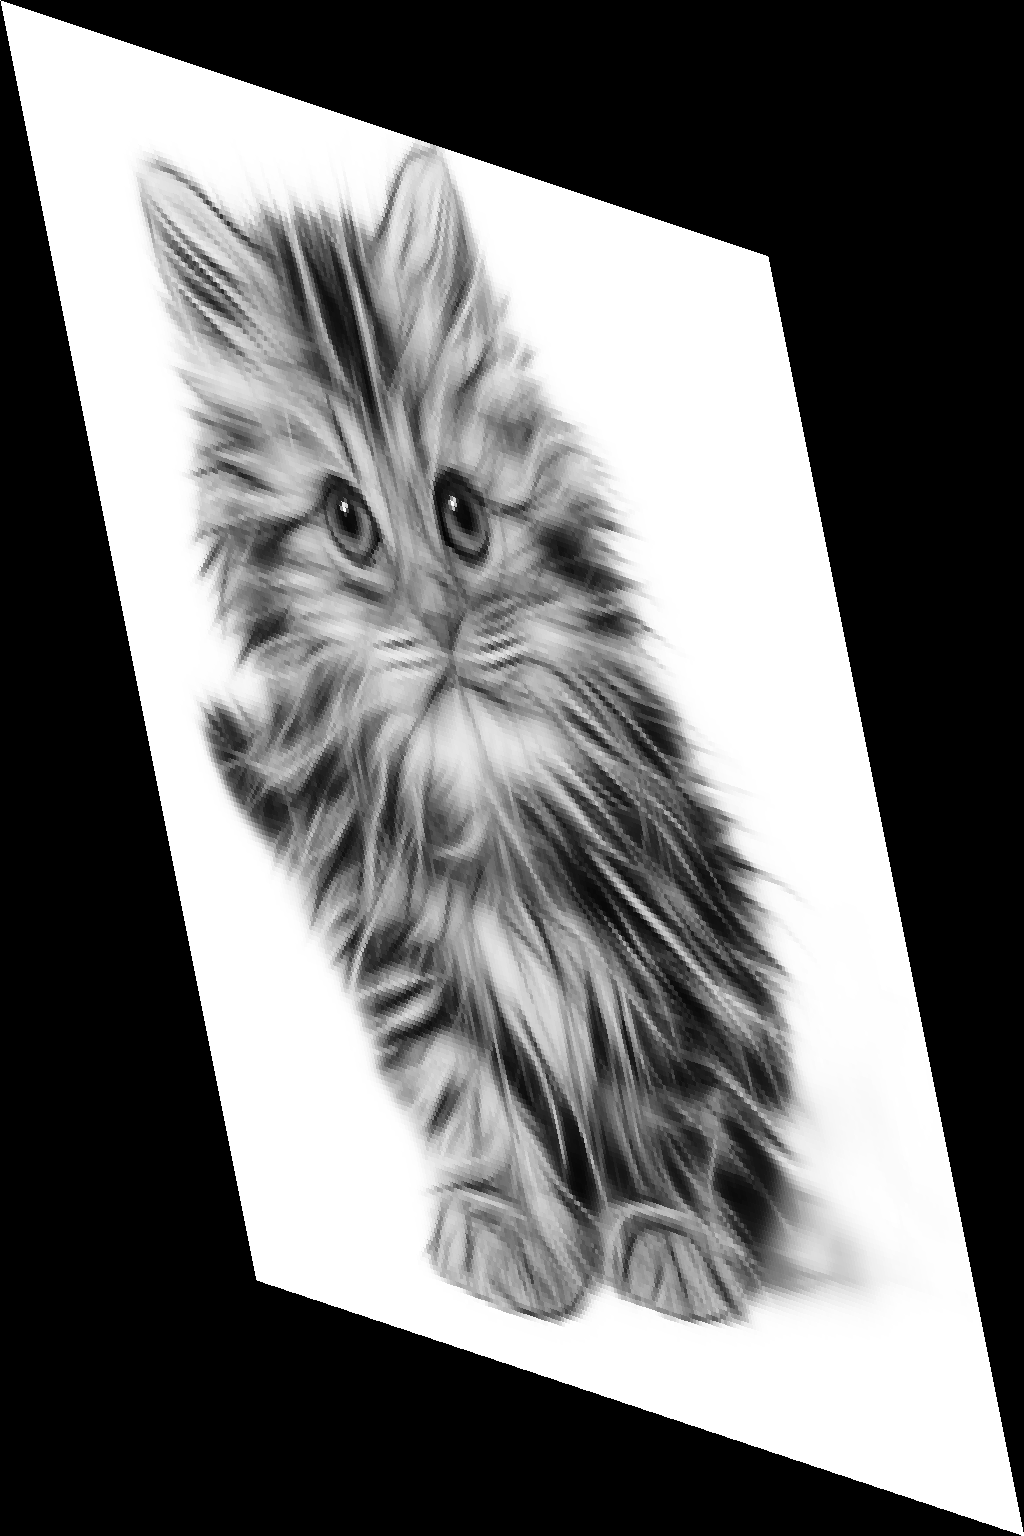
\includegraphics[scale=\myscale,scale=0.1]{png/chat_transfo}
	\end{minipage}
	 \end{center}
 
 	Voici comment programmer cette fonction.
 	
 	\textbf{Première étape : taille de la nouvelle matrice.}
 	
 	On identifie la matrice $M$ de taille $n \times  p$ à une image rectangulaire. Les quatre coins de cette image ont pour coordonnées  $P_0 = \begin{pmatrix}0\\0\end{pmatrix}$,
 	$P_1 = \begin{pmatrix}p\\0\end{pmatrix}$, $P_2=\begin{pmatrix}p\\n\end{pmatrix}$, $P_3=\begin{pmatrix}0\\n\end{pmatrix}$.
 	Calcule les coordonnées $P'_i = \begin{pmatrix}x_i\\y_i\end{pmatrix} = T \cdot P_i$ des coins transformés : ce sont les sommets d'un parallélogramme (ce n'est pas toujours un rectangle).
 	
 	% [[dessin]] 	
 	
 	On note :
 	$$x_{\min} = \min(x_0,x_1,x_2,x_3) \qquad \text{ et } \qquad x_{\max} = \max(x_0,x_1,x_2,x_3)$$
 	$$y_{\min} = \min(y_0,y_1,y_2,y_3) \qquad \text{ et } \qquad y_{\max} = \max(y_0,y_1,y_2,y_3)$$
 	
 	L'image transformée est incluse dans le rectangle défini par $(x_{\min},x_{\max},y_{\min},y_{\max})$ !
 
\myfigure{0.9}{\tikzinput{fig-transfo-7}}		
 	
 	On retient :
 	\begin{itemize}
 		\item le nombre de lignes de la matrice transformée est $n' = y_{\max}-y_{\min}$ (c'est la hauteur de l'image transformée), 		
 		\item le nombre de colonnes de la matrice transformée est $p' = x_{\max}-x_{\min}$ (c'est la largeur de l'image transformée).
 	\end{itemize} 
 	
 	\textbf{Seconde étape : formule de la transformation.}
 	
 	La nouvelle matrice $N$ sera une matrice de taille $n'\times p'$. 	
 	
 	Pour savoir combien vaut le coefficient $N[i'][j']$, il faut trouver le coefficient $M[i][j]$ correspondant dans la matrice de départ. 
 	(Autrement dit : la nouvelle l'image est de taille $n'\times p'$, le pixel $(i',j')$ est de niveau de gris $N[i'][j']$ qui se calcule en fonction du niveau de gris $M[i][j]$.) 
 	
 		
 	Il faut donc utiliser la matrice inverse $T^{-1}$. En plus il faut effectuer une translation de vecteur
 	$\left(\begin{smallmatrix}x_{\min}\\y_{\min}\end{smallmatrix}\right)$ pour recentrer l'origine.	
 	Ce qui donne :
 	$$\begin{pmatrix}j\\i\end{pmatrix} = T^{-1}  \begin{pmatrix}j'+x_{\min}\\i'+y_{\min}\end{pmatrix}$$
 	et ensuite simplement :
 	$$N[i'][j'] = M[i][j]$$
 	
 	\emph{Exemple.} Voici une dilatation avec des coefficients non entiers : le nombre de colonnes passe de $3$ à $4$ (facteur $k_x = \frac43$), le nombre de lignes est doublé ($k_y=2$).  
 	$$T = \begin{pmatrix}\frac43&0\\0&2\end{pmatrix}\qquad
 	M = \begin{pmatrix}
 	 1 & 2 & 3 \\
 	4 & 5 & 6 \\
 	7 & 8 & 9 \end{pmatrix}\qquad
 	N = \begin{pmatrix}
 	1 & 1 & 2 & 3 \\ 
 	1 & 1 & 2 & 3 \\ 
 	4 & 4 & 5 & 6 \\ 
 	4 & 4 & 5 & 6 \\ 
 	7 & 7 & 8 & 9 \\ 
 	7 & 7 & 8 & 9 
 	\end{pmatrix}$$
 		
\end{enumerate}

Tu peux maintenant transformer des images.
	
\end{activite}


\end{document}
